% An overview of the experiment is shown in figure \ref{fig:schedule}
% \begin{figure}[h]\centering
%     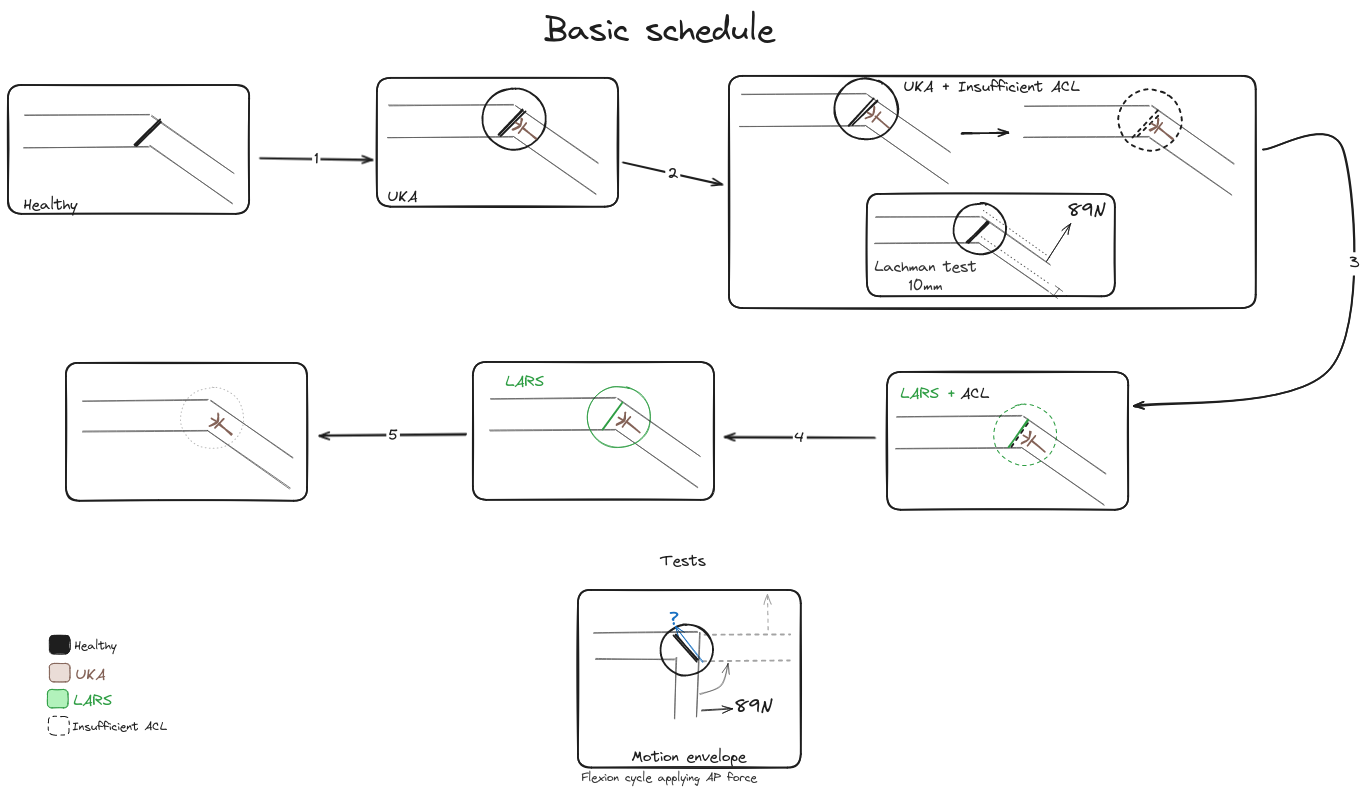
\includegraphics[width=\textwidth]{figures/schedule}
% \caption{Schedule overview}
% \label{fig:schedule}
% \end{figure}

% \subsection{Test: Biomechanics envelope}\label{sec:nkna}
% Setup + Test take approximately 1 hour.
% \begin{enumerate}
%     \item Knee placed on the rig with 0\degree flexion.
%     \item Posterior tibia force of \SI{89}{N} applied along the joint line.
%     \item Flex from 0\degree to 90\degree, tracking kinematic data (tibial internal rotation, valgus/varus rotation, proximal displacement, etc).
%     \item Anterior tibia force of \SI{89}{N} applied along the joint line.
%     \item Flex from 90\degree to 0\degree, tracking kinematic data.
%     \item Repeat 3 times.
% \end{enumerate}

% \subsection{Schedule}

\begin{enumerate}[start=0,label={Day \arabic*}:]
    \item \textbf{Exp 1:} Native knee (healthy ACL) test 
    \item \begin{enumerate}
            \item \textbf{Surg 1: 60 min} UKA. 
            \item \textbf{Exp 2: 60 min} UKA test 
            \item \textbf{Surg 2: 15 min} Pie-crust/partial transection of ACL while still mounted on the rig. Aim for 10 mm AP laxity. Laxity measured by the robot.
            \item \textbf{Exp 3: 30 min} UKA + deficient ACL test
            \item \textbf{Surg 3: 60 min} ACL augmentation \todo{Exact technique is an open question}
            \item \textbf{Exp 4: 60 min} UKA + augmented ACL test
            \item \textbf{Surg 4: 10 min} Transect ACL while still mounted on the rig
            \item \textbf{Exp 5: 30 min} UKA + reconstructed ACL test
            \item \textbf{Surg 5: 10 min} Remove synthetic ligament
            \item \textbf{Exp 6: 60 min} UKA and no ACL test
        \end{enumerate}
